\documentclass[12pt]{article}

\parindent=.25in
\setlength{\oddsidemargin}{0pt}
\setlength{\textwidth}{440pt}
\setlength{\topmargin}{0in}

\usepackage{amsmath}
\usepackage{amsfonts}
\usepackage[dvips]{graphicx}
\usepackage{verbatim}
\usepackage{appendix}

% Title Page
\title{OurCompany Case Study Solution}
\author{Mengqi Zong}

\begin{document}
\maketitle

% No Indentation
\setlength{\parindent}{0in}

{\bf 1. Which Campaign was the most profitable?} \\

First, we give three ways to define ``most profitable'':

\begin{enumerate}
\item Profit

	\begin{equation*}
		\text{Profit} = \text{Adv Cost} - \text{Pub Earning} - \text{Data Segment Cost}
	\end{equation*}

	Given the data, which campaign generates the greatest profit for OurCompany.

\item Profit/Impressions

	\begin{eqnarray*}
		\frac {\text{Profit}}{\text{Impressions}}
		&=& \frac {\text{Adv Cost} - \text{Pub Earning} - \text{Data Segment Cost}}{\text{Impressions}} \\
		&=& \frac {\text{Clicks} \cdot \text{Price}_{\text{adv}} - \text{Clicks} \cdot \text{Price}_{\text{pub}}  - \text{Impressions} \cdot \text{Price}_{\text{data}}}{\text{Impressions}} \\
		&=& \text{CTR} \cdot \text{Price}_{\text{adv}} - \text{CTR} \cdot \text{Price}_{\text{pub}} - \text{Price}_{\text{data}} \\
		&=& \text{CTR} \cdot (\text{Price}_{\text{adv}} - \text{Price}_{\text{pub}}) - \text{Price}_{\text{data}}
	\end{eqnarray*}

	When OurCompany delivers the same amount of impressions for each campaign, which campaign generates the greatest profit for OurCompany.
	
\item ROI

	\begin{eqnarray*}
		\text{ROI} &=& \frac {\text{Profit}} {\text{Cost}} \\
				   &=& \frac {\text{Profit}} {\text{Pub Earning} + \text{Data Segment Cost}}
	\end{eqnarray*}
	
	When OurCompany pays the same amount of money for each campaign, which campaign generates the greatest profit for OurCompany.
\end{enumerate}

Here are the results using three different criteria:

\begin{itemize}
\item Profit

	Campaign3. The Profit is \$21500.58.
\item Profit/Impression

	Campaign3. The Profit/Impression is 0.000844578.
\item ROI

	Campaign3. The ROI is 117.93\%.
\end{itemize}

{\bf 2. Which publisher was the most profitable?} \\

Similar to Question 1, we give results using three different criteria:

\begin{itemize}
\item Profit

	PubID 737367. The Profit is \$26723.12.
\item Profit/Impression

	PubID 737367. The Profit/Impression is 0.003066583.
\item ROI

	PubID 11911998. The ROI is 322.92\%.
\end{itemize}

{\bf 3. What is the average CTR\% for Campaign1?} \\

The average CTR\% for Campaign1 is 0.1519153\%. \\

{\bf 4. On the publisher by publisher basis, which segments showed lift and performance over RON impressions. Would you say that segments actually cause differentiation in performance? Use CTR\% as the primary performance indicator.} \\

The CTR\% for each ``Pub ID / Segment'' combination is shown in spreadsheet ``P4\_CTR'' of file ``dataset.xlsx''. Note that ``INV'' means there is no such ``Pub ID / Segment'' combination in the original data. \\

We compared the CTR\% of RON with that of other segments on the publisher by publisher basis. There are 782 of 1565 segments showed lift and performance over RON impressions, while 783 of 1565 segments didn't. \\

If segments don't cause differentiation in performance, then the probability of one segment showed lift and performance over RON should be 0.5. In this case, we can use proportional test to test this hypothesis. Here is the test result from R:

\begin{verbatim}
        1-sample proportions test with continuity correction

data:  782 out of 1565, null probability 0.5
X-squared = 0, df = 1, p-value = 1
alternative hypothesis: true p is not equal to 0.5
95 percent confidence interval:
 0.4746210 0.5247416
sample estimates:
        p
0.4996805
\end{verbatim}

The proportional test showed that the probability of segments showed lift and performance over RON is 0.5 (p-value = 1). \\

In conclusion, segments actually don't cause differentiation in performance. \\

{\bf 5.	Is there a single data segment that is the most effective across publishers based on CTR\%? Is it effective for all publishers?} \\

The most efficient segment is "Cell Phone", but it is not effective for all publishers. \\

We first calculated the average CTR\% for each data segment. The segment which has the greatest average CTR\% is ``Cell Phones''. Its average CTR\% is 2.259422\%. \\

We also counted the number of times that each segment is in the top 3 greatest CTR\% segments for each publisher. It turns out that "Cell Phone" has 33 of 107 times in the top 3 for all publishers. And 33 is the highest count among data segments. \\

In conclusion, the most efficient segment is "Cell Phone", but it is not effective for all publishers. \\

{\bf 6. Is click through rate metric by publisher normally distributed in the data set?} \\

The CTR\% by publisher is not normally distributed in the data set. \\

The CTR\% for all publishers are listed in spreadsheet "P2\&P6". The QQ plot for all the 164 CTR\% is shown in Fig~\ref{fig:qq}. As we can see, the click through rate metric by publisher is not normally distributed in the data set. \\

\begin{figure}[ht!]
  \centering
  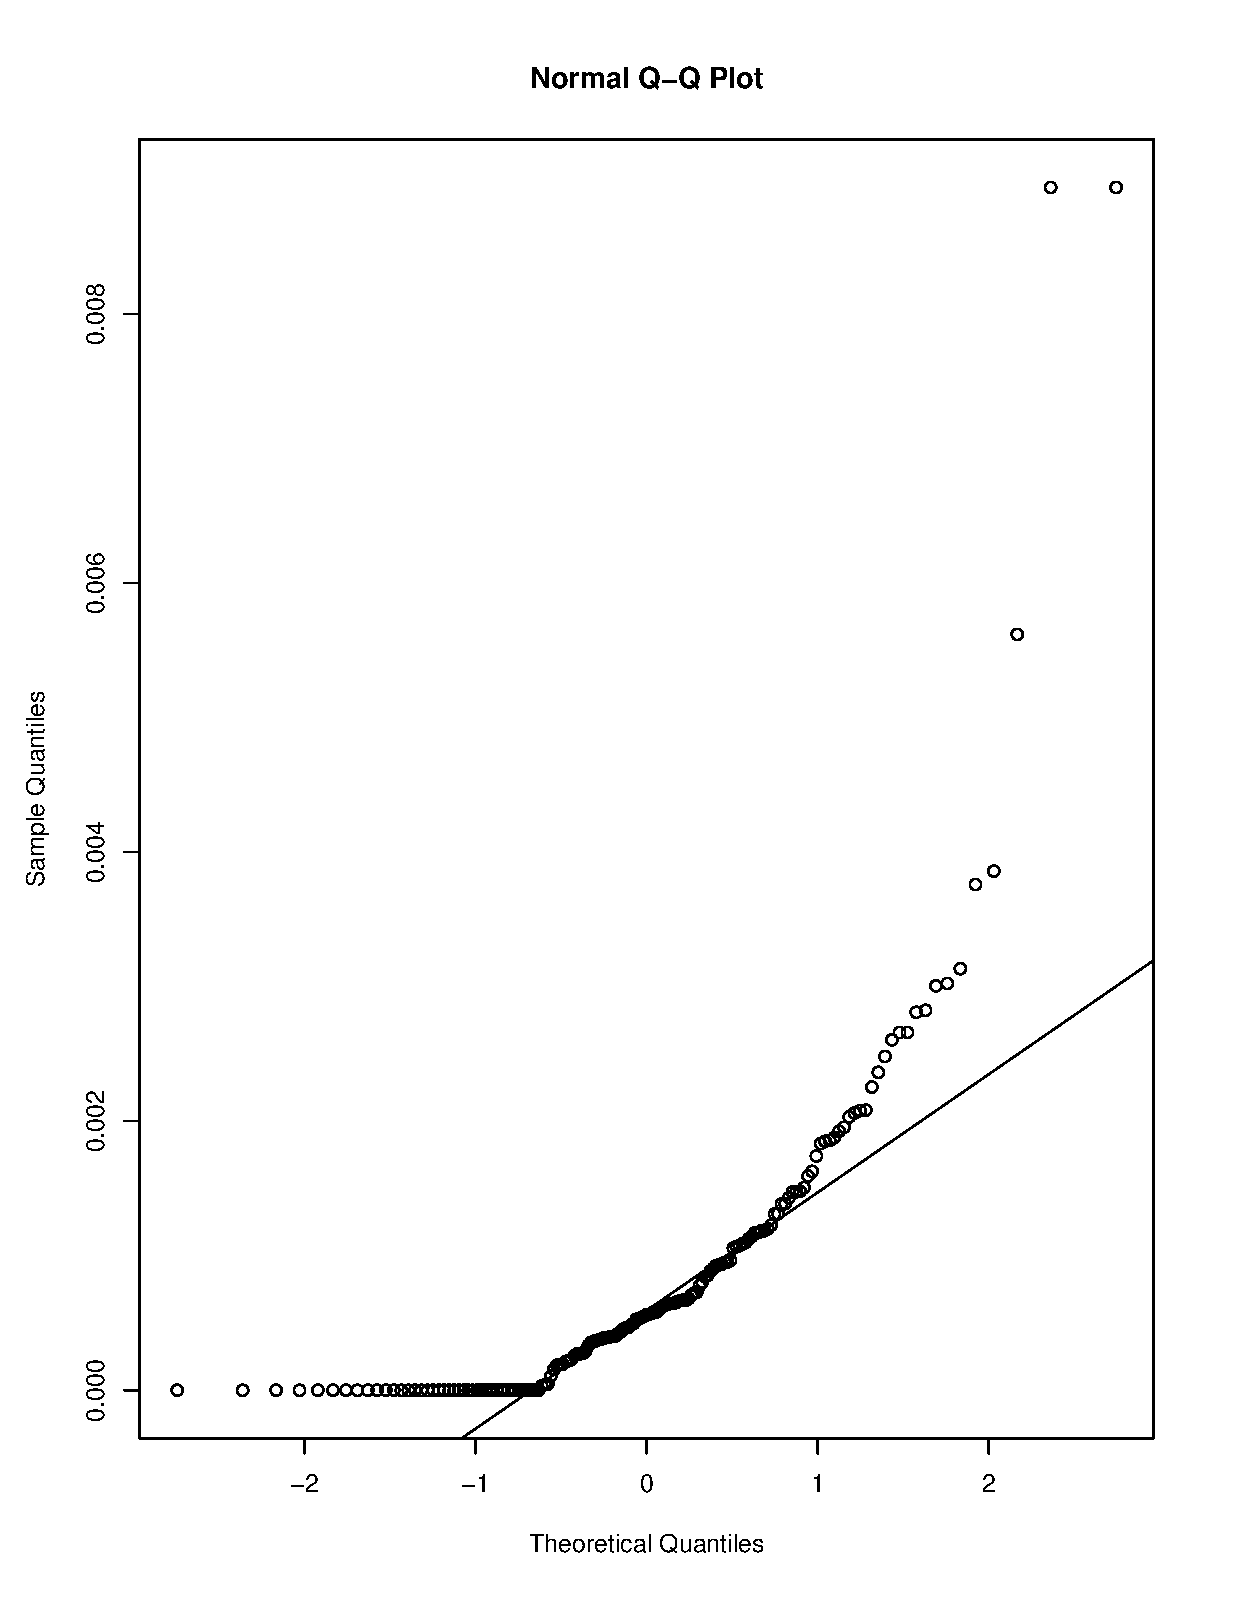
\includegraphics[width=0.8\textwidth]{qq}
  \caption{Q-Q plot for CTR\% \label{fig:qq}}
\end{figure}

We also used Shapiro-Wilk normality test. Here is the test result from R:

\begin{verbatim}
        Shapiro-Wilk normality test

data:  CTR
W = 0.652, p-value < 2.2e-16
\end{verbatim}

As we can see, the data is not normally distributed ($p-value < 0.05$). \\

{\bf 7. What combination of campaign/ publisher would result in the most profitable outcome? How much performance is lost on campaign level? Constraint here is to deliver the same number of impressions for each campaign.}



\end{document}
